\documentclass[times]{itmo-student-thesis}

%% Опции пакета:
%% - specification - если есть, генерируется задание, иначе не генерируется
%% - annotation - если есть, генерируется аннотация, иначе не генерируется
%% - times - делает все шрифтом Times New Roman, собирается с помощью xelatex
%% - languages={...} - устанавливает перечень используемых языков. По умолчанию это {english,russian}.
%%                     Последний из языков определяет текст основного документа.

%% Делает запятую в формулах более интеллектуальной, например:
%% $1,5x$ будет читаться как полтора икса, а не один запятая пять иксов.
%% Однако если написать $1, 5x$, то все будет как прежде.
\usepackage{icomma}

\newcommand{\Edelta}{$E[_{\Delta} X_t| X_t=I]$}
\newcommand{\EY}{E[Y_t| X_t = I]}
\newcommand{\EZdelta}{$E[Z_t, X_t=I]$}
\newcommand{\prn}{\frac{r}{n}}

%% Один из пакетов, позволяющий делать таблицы на всю ширину текста.
\usepackage{tabularx}
\usepackage{enumitem,kantlipsum}
\usepackage{graphicx}
\graphicspath{{pictures/}}

%% Данные пакеты необязательны к использованию в бакалаврских/магистерских
%% Они нужны для иллюстративных целей
%% Начало
\usepackage{tikz}
\usetikzlibrary{arrows}


%% Указываем файл с библиографией.
\addbibresource{bachelor-thesis.bib}

\begin{document}

    \studygroup{M3437}
    \title{Теоретическое исследование эволюционного алгоритма (1+1) на динамических псевдобулевых задачах оптимизации}
    \author{Торопин Константин Игоревич}{Торопин К. И.}
    \supervisor{Максим Викторович Буздалов}{Буздалов М.В.}{к.т.н.}{}
    \publishyear{2021}
%% Дата выдачи задания. Можно не указывать, тогда надо будет заполнить от руки.
%%\startdate{01}{сентября}{2018}
%% Срок сдачи студентом работы. Можно не указывать, тогда надо будет заполнить от руки.
%%\finishdate{31}{мая}{2019}
%% Дата защиты. Можно не указывать, тогда надо будет заполнить от руки.
%%\defencedate{15}{июня}{2019}

    \secretary{Павлова О.Н.}

%% Задание
%%% Техническое задание и исходные данные к работе

%%% Содержание выпускной квалификационной работы (перечень подлежащих разработке вопросов)
    \plannedcontents{\begin{enumerate}
                         \item Постановка задачи
                         \item Поиск плато
                         \item Оценки скорости нахождения первого оптимума
                         \item Проверка гипотез на реальных данных
    \end{enumerate}}

%%% Исходные материалы и пособия

%%% Цель исследования
    \researchaim{Анализ динамического алгоритма $(1+1)EA$ на задаче $OneMax$}
    \researchaim{Разработка теоретической базы для анализа эволюционных алгоритмов с динамически изменяемыми функциями}

%%% Задачи, решаемые в ВКР
    \researchtargets{\begin{enumerate}
                         \item Нахождение плато в зависимости от динамики;
                         \item Проработка теории для анализа времени работы алгоритмов
                         \item Проверка теории на практике
    \end{enumerate}}

%%% Использование современных пакетов компьютерных программ и технологий
    \addadvancedsoftware{Интегрированная среда разработки PyCharm}{\ref{ch:проверка-гипотез}
    \addadvancedsoftware{Язык программирования Python}{\ref{ch:проверка-гипотез}}}

%%% Краткая характеристика полученных результатов
    \researchsummary{
        Проанализирован алгоритм (1 + 1)EA на задаче OneMax с динамическими изменениями, а так же была расширена теоретическая база эволюционных алгоритмов на динамических псевдобулевых задачах оптимизации\\
        .}

%%% Гранты, полученные при выполнении работы
    \researchfunding{Грантов и других форм государственной поддержки и субсидирования в процессе в процессе выполнения не предусматривалось.}

%%% Наличие публикаций и выступлений на конференциях по теме выпускной работы
    \researchpublications{Публикации и выступления, связанные с данной работой, отсутствуют.}

%% Эта команда генерирует титульный лист и аннотацию.
    \maketitle{Бакалавр}

%% Оглавление
    \tableofcontents

%% Макрос для введения. Совместим со старым стилевиком.

    \startprefacepage

    В практике применения эволюционных алгоритмов нередко встречаются динамические задачи оптимизации, в рамках которых оптимизируемая функция изменяется со временем.
    В теоретическом анализе времени работы эволюционных алгоритмов не так много работ уделяется этим задачам.
    И в этих работах центральным ставится вопрос может ли быть достигнут оптимум между изменениями функции приспособленности, а то, как в промежутке меняется значение приспособленности, не особо рассматривается, за вычетом приспособленностей, крайне близких к оптимуму.
    В частности не решается вопрос что должно происходить с различными способами адаптации параметров, которые применяются для повышения эффективности алгоритмов. Поэтому задача анализа алгоритма (1 + 1) на динамических псевдобулевых задачах оптимизации является актуальной.


    \chapter{Пояснительная записка}

    Эволюционные алгоритмы могут применяться для поиска экстремума функции.

    Однако в теории эволюционных алгоритмов существует проблема, которая заключается в том, что функция в процессе поиска экстремума может изменятся.
    Примером такой задачи может быть поиск оптимального маршрута в городе - искомый маршрут в зависимости от времени может отличаться.
    Поэтому возникает потребность проанализировать алгоритмы учитывая динамическое преобразование функции.
    Для начала был взят алгоритм (1 + 1) на задаче $OneMax$.

    Данный алгоритм был выбран потому что это наиболее понятная и простая задача для анализа и часто является отправной точкой для исследования.

    OneMax - задача поиска минимума функции количества несовпадающих бит с некоторым вектором $f_{max}$, длина которого $n$.

    Алгоритм (1 + 1) решает её следующим образом - берётся случайный вектор длины $n$ и далее итеративно мутируется - каждый бит независимо меняется с некоторой вероятностью $\frac{r}{n}$ ($r$ рассматривается в данном исследовании $o(1)$ по отношению к $n$).
    Если количество совпадающих бит увеличивается, берётся мутируемый.
    Добавим следующую динамику для задачи - пусть каждые $T$ итераций алгоритма вектор $f_{max}$ меняет один случайный бит.
    Существуют несколько статей на похожую тему  \cite{dinamically_1} и \cite{dinamically_2} где также исследуется вопрос скорости работы динамических алгоритмов, однако в этих статьях нет исследований самого поведения алгоритма.
    В рамках исследования были выявлены две ситуации - когда $T$ слишком мала, то алгоритм "застревает"  на некотором значении, расстояние до $f_{max}$ колеблются на уровне некоторого $с \cdot n$.
    Значение $c$ будем называть точкой стабилизации или плато.
    То есть в этой ситуации с некоторого момента примерное отношение бит которые не совпадают с вектором $f_{max}$ ко всем битам будет равна $c$.
    Вторая ситуация - $T$ оказывается достаточно большой, что алгоритм доходит до нужного оптимума, однако медленнее чем если бы динамики не было.
    Помимо этого был рассмотрена ситуация когда алгоритм не заканчивается на достижении оптимума (что вполне можно увидеть на реальных задачах).
    Тогда будет разумным вопрос - какая вероятность, что при изменении одного бита алгоритм успеет найти новый оптимум до следующего изменения.

    По первому случаю был установлен факт, что значение $c$ не зависит от параметра $T$ (если $n > 1/c$), это значит что если мы фиксируем какое-то значение $T$, то насколько сильно мы бы не увеличивали $n$, значение $c$ будет оставаться тем же.
    Были найдены некоторые оценки на значение $c$, а также теоретически обоснован факт почему алгоритм фиксируется и почти не уходит от этого значения.

    Что касается второго случая - асимптотика EA-алгоритмов обычно оценивается с помощью некоторых теорем которые несут общее название drift-analysis.
    Были взяты теоремы Additive Drift и Variable Drift и рассмотрены с точки зрения того, что математическое ожидание изменения функции на некоторых шагах отличается от обычного.
    Если рассматривать данную конкретную задачу, то в ней каждые $K$ шагов математическое ожидание будет отличаться на некоторое значение $\leq 1$.
    Эти теоремы в дальнейшим могут помочь исследовать скорость нахождения первого оптимума и в более сложных алгоритмах в которых будет введена динамика.
    С помощью видоизмененных теорем была доказано, что если $T$ больше некоторого значения, то асимптотика алгоритма не изменится, то есть останется $O(n \cdot log(n))$

    Экспериментальные данные показывают, что плато находится на тех значениях, которые предсказывает теория.

    \chapter{Теоретическое исследование}

    \section{Постановка задачи}

    Для начала рассмотрим базовую задачу $OneMax$ в том, чтобы найти заданный вектор, когда у нас есть только "черный ящик" который говорит сколько бит совпадает с оптимальным вектором.
    Суть базового алгоритма $(1 + 1)EA$ в том берём случайный вектор, и каждую итерацию изменяем каждый бит независимо с некоторой вероятностью $\frac{r}{n}$, где $n$ - длина вектора, а $r$ - некоторая константа
    Более наглядно показано с помощью псевдокода
    \begin{algorithm}
        \caption{OneMax (1 + 1)EA}\label{alg:Example}
        \begin{algorithmic}[1]
            \Require {$x_{max}$ - required vector; $n$ — dimensionality of vector; $r$ - constant}
            \State Sample first individual $x$ randomly
            \State Calculate fitness of $x$: $f_{best} \leftarrow samebits(x, x_{max})$
            \While{$x \neq  x_{max}$}
                \State $y \leftarrow mutate(x, \frac{r}{n})$
                \State $f_y \leftarrow samebits(y)$
                \If{$f_y > f_{best}$}
                    \State $x \leftarrow y$
                    \State $f_{best} \leftarrow samebits(y, x_{max})$
                \EndIf
            \EndWhile
            \algstore{bkbreak}
        \end{algorithmic}
    \end{algorithm}
    \begin{algorithm}
        \caption{OneMax (1 + 1)EA with dynamic}\label{alg:Example2}
        \begin{algorithmic}[1]

            \algrestore{bkbreak}
            \Require {$x^{opt}$ - required vector; $r$ - constant; $T$ - constant}
            \State Sample first individual $x$ randomly
            \State Calculate fitness of $x$: $f_{best} \leftarrow samebits(x, x_{max})$
            \State $i \leftarrow 1$
            \While{$x \neq  x^{opt}$}
                \If{$i \mod T  = 0$}
                    \State $x_{max} \leftarrow change(x^{opt})$
                \EndIf
                \State $y \leftarrow mutate(x, \frac{r}{n})$
                \State $f_y \leftarrow samebits(y)$
                \If{$f_y > f_{best}$}
                    \State $x \leftarrow y$
                    \State $f_{best} \leftarrow samebits(y, x^{opt})$
                \EndIf
            \EndWhile

        \end{algorithmic}
    \end{algorithm}

    Суть алгоритмов $(1 + 1)EA$ и задачи $OneMax$ детально расписана в \cite{base_one_max_1} и \cite{base_one_max_2}.

    Далее введём для данного алгоритма динамику схожую с той, которую вводят в \cite{optima_1} \cite{optima_2}. Раз в $T$ итераций алгоритм случайным образом изменяет в необходимом векторе ровно один бит.


    В ходе практического анализа алгоритма была обнаружена закономерность, что алгоритм при некоторых значениях параметра $T$ алгоритм "останавливается"  в некоторых точках.

    Для дальнейшего анализа нам потребуются обозначения:
    \begin{enumerate}
        \item[] $(x_t^{opt})_{t \in N}$ - оптимальный вектор, который алгоритм пытается найти на итерации $t$.
        \item[] $x_0^{opt}$ считаем равным изначальному искомому вектору
        \item[] Множество всевозможных пар ${x_t, x_t^{opt}}$ будет задавать пространство исходов $\Omega$ , вероятность конкретного исхода как и вся $\sigma$-алгебра естественным образов выводится из фильтрации, которую пораждает случайный процеесс.
        \item[] Таким образом построено вероятностное пространство $(\Omega, \mathcal{F}, \mathbb{P})$.
        \item[] $samebits(a, b)$ - количество совпадающих бит у двух векторов.
        \item[] $X_t := samebits(x_t, x_t^{opt})$, последовательность случайных величин обозначающих количество совпадающих бит текущего вектора на итерации $t$.
        \item []$Y_t$ - случайная величина, обозначающая прирост величины $X_t$ за счёт изменения вектора $x_t$.
        Формально $Y_t := $\begin{cases}
                               samebits(x_t, x_{t - 1}^{opt}) - X_{t - 1}, &\mbox{if } t > 0 \\
                               0, &\mbox{if } t \eq 0
        \end{cases}.
        \item[] $Z_t$ - случайная величина, обозначающая уменьшение величины $X_t$ за счёт изменения $x_t^{opt}$.
        Формально $Z_t := $\begin{cases}
                               samebits(x_{t}, x_{t}^{opt}) - samebits(x_{t}, x_{t - 1}^{opt}), &\mbox{if } t > 0 \\
                               0, &\mbox{if } t \eq 0
        \end{cases}
        \item[] Очевидно что в рамках данной задачи $Z_t = \{0, -1\}$ для всех $t$.
        \item[] Так же можно увидеть что $X_t = X_{t - 1} + Y_t + Z_t$.
    \end{enumerate}

    Небольшая ремарка: в дальнейших рассуждениях будут использоваться формулы вида $E[X_{t+1} = a | x_t = I]$ то есть в них будет опускаться фильтрация, хотя она, конечно, неявно подразумевается.
    Введём обозначения $p = \frac{r}{n}$, $q = 1 - p$.
    \section{Поиск плато}

    В ходе практического исследования алгоритма был установлен факт, что для некоторых $T$ значение алгоритм останавливается на некотором значении и не может далеко уйти за эти рамки.
    Назовём значение этой точки "плато" и будем искать его в следующей точке: пусть $I$- количество совпадающий бит, $n$ - длина массива где математическое ожидание "подняться вверх" то есть на сколько больше бит будет будет равняться оптимальному будет равно значению $\frac{1}{T \cdot  n}$.
    Физический смысл этого можно понять так: пусть мы рассматриваем задачу, когда динамика может происходить каждый раз, но с вероятностью 1/T.
    Данная задача также исследуется в \cite{noise_2} \cite{noise_3}.
    Вероятность того, что динамика ухудшит ответ будет $\frac{I}{T \cdot n}$ и математическое ожидание будет процесса динамики будет равно этому же $\frac{I}{T \cdot n}$.
    Так что суммарное математическое ожидание будет равно 0.

    На самом деле задача стоит другим образом и честная оценка $E[X_{t+T} - X_t, x_t = I]$ через T итераций будет ниже чем $T \cdot \EY$ потому что она убывает от роста I, но заглядывая в будущее, окажется что этого приближения достаточно, и уйти от данной точки на линейную длину алгоритму будет экспоненциально сложно.

    Пусть в данный момент у алгоритма величина $X_t = I$, то есть количество бит текущего, которые совпадают с текущим оптимальным вектором.
    Введём обозначения - для конкретной $I$
    \begin{gather*}
        Bin(m, n) \equiv C_m^n \cdot p^{m} \cdot q^{n - m} = C_m^n \cdot p^{m} \cdot q^{n - m}\\
        A(i) \equiv Bin(i, I)\\
        Q(i) \equiv Bin(i, n - I)\\
        с = \frac{I}{n}\\
    \end{gather*}

    Значение $c$ можно рассматривать как процент правильных бит.
    Значение $A(i)$ как вероятность что среди $I$ бит произойдёт ровно $i$ изменений.
    Значение $Q(i)$ как вероятность что среди $n - I$ бит произойдёт ровно $i$ изменений.

    Так как вероятность изменения значения вектора ровно на $i$ равна вероятности того что среди ещё не найденных бит изменится ровно $k$ бит, а в найденных изменится $k - i$ для всех возможных $k$.

    \begin{gather*}
        P(Y_t = i|X_t=I) = \sum_{j=1}^{\min(I - i, n - I - i)} A(i + j)Q(i)
    \end{gather*}

    Давайте рассматривать только такие $I$ что
    \begin{gather*}
        c > 0.5 \\
        r = O(1), при n \rightarrow \infty
    \end{gather*}

    Очевидно что рассматривать алгоритм в тех случаях, когда $c < 0.5$ не имеет смысла, так как уже начальное приближение задачи при инициализации вектора будет иметь математическое ожидание количества совпадающих бит уже $\frac{n}{2}$.
    По поводу второго приближения, все изучения задачи $OneMax$ всегда используют $r = o(1)$, а ещё чаще равному 1.

    Заметим что
    \begin{gather*}
        P(Y_t = i|X_t=I) = \sum_{j=1}^{I - i} A(i + j)Q(i)
    \end{gather*}

    Тогда значение $\EY$ можно расписать в виде:
    $\EY = \sum_{i=1}^I i \cdot \sum_{j=1}^{I - i} A(i + j)Q(i) = \sum_{i=1}^I Q(i) \sum_{j=i}^{I} j \cdot A(j - i) =$
    \begin{align*}
        = Q(0)A(1) + && 2\cdot Q(0)A(2) && + 3\cdot Q(0)A(3) && + {}\ldots{} && + I\cdot Q(0)A(I) + & \\
        && Q(1)A(2)   && + 2\cdot Q(1)A(3) && + {}\ldots{} && + (I-1)\cdot Q(1)A(I)  + &\\
        && && && + {}\ldots{} && + \vdotswithin{A(I)Q(n - I)} &
    \end{align*}

    Так как $\sum_{j=1}^{I} j \cdot A(j)$ это определение матожидание случайной величины $A$, которая равна $pI$.

    Заметим что первая строка равна

    $\tau^* \equiv Q(0) \cdot \sum_{j=1}^{I} j \cdot A(j) = Q(0) \cdot pI = q^{n - I} \cdot c \cdot r$. Это будет нашей нижней оценкой на $\EY$

    Далее оценим сумму остальных строк.
    Оценим сверху для каждой строки во сколько изменяется элемент в строке относительно предыдущего, взяв отношение элемента в строке $j + 1$ и поделим на элемент в строке $j$:

    Для строки $i \geq 2$

    \begin{gather*}
        \frac{(j + 1)\cdot Q(i)\cdot A(i + j + 1)}{j\cdot Q(i) \cdot A(i + j)} \\
        = \frac{j + 1}{j} \cdot \frac{I!}{(I - (i + j + 1))! \cdot (i + j + 1)!} \cdot p^{I - (i + j + 1)} q^{i + j + 1} \cdot\\
        \cdot \frac{(I - (i + j))! \cdot (i + j)!} {I!} \cdot \frac{1}{p^{I - (i + j)} q^{i + j}} \\
        = \frac{j + 1}{j} \cdot \frac{I - i - j}{i + j + 1} \cdot (\frac{q}{p} = \frac{r \cdot n}{n \cdot (n - r)} = \frac{r}{n - r}) \\
        =  \frac{j + 1}{j \cdot (i + j + 1)} \cdot  \frac{c\cdot (n - r) + c\cdot r - i - j)}{n - r} \cdot r \leq \\
        \leq \frac{1}{2} \cdot \frac{c\cdot (n - r)}{n - r} \cdot r + o(1) \approx \frac{c \cdot r}{2}
    \end{gather*}

    Все попытки анализа данной модели для $r$ равной произвольной константе от $n$ не увенчались успехом, скорее всего для анализа необходимо использовать модель по аналогии с той, которая делалась в \cite{markov_chain}

    Если принять гипотезу что $r < 2$, тогда каждая строка $i$:
    \begin{gather*}
        a_i \equiv \sum_{j = 1}^{I - i} (j \cdot Q(i) \cdot A(i + j)) \leq \\
        \leq \sum_{j = 1}^{inf} (Q(i) \cdot A(i + 1) \cdot (\frac{c \cdot r}{2})^{j}) \\
        = Q(i) \cdot A(i + 1) \cdot \frac{1}{1 - \frac{c \cdot r}{2}}
    \end{gather*}

    Аналогично сравним первые элементы рядов $i$ и $i + 1$:
    \begin{gather*}
        \frac{Q(i + 1) \cdot A(i + 2)}{Q(i) \cdot A(i + 1)} = \frac{(n - I - i) \cdot (I - i - 1)}{(i + 1) \cdot i} \cdot (\frac{r}{n - r})^2 \\
        \leq \frac{(1 - c) \cdot (n - 1)2 \cdot c \cdot r^2}{(n - r)^2} = c \cdot (1 - c) \cdot r^2
    \end{gather*}

    Получившийся коэффициент сходится благодаря тому что $c \cdot (1 - c) < 1/4$, а $r < 2$ как мы приняли.

    Аналогично получается геометрическая прогрессия, которая сходится, теперь посчитаем сумму всех рядов:

    \begin{gather*}
        Q(1)A(2) \cdot \frac{1}{1 - c \cdot (1 - c) \cdot r^2 } \cdot \frac{1}{1 - c \cdot r/2} = \\
        =\frac{(n - I)\cdot I\cdot (I - 1)}{2} \cdot p^3 \cdot q^{n - 3} \cdot constants \leq\\
        \leq c^2 \cdot r^3 \cdot q^{n - 3} = (q^{n - I} \cdot c \cdot r) \cdot  (q^{I - 3} \cdot c \cdot r^2)  = \tau^* \cdot (q^{I - 3} \cdot c \cdot r^2)
    \end{gather*}
    Значение $constants < 1$ его можно использовать, чтобы брать более качественные оценки на $c_{lower}$ о котором будет говорится позже.

    Оценки $\tau^*$:  \\
    Введем значение $\tau \equiv \exp(-r + r\cdot c) \cdot c \cdot r$
    \begin{gather*}
        \tau^* = q^{n - I} \cdot c \cdot r = (1 - r/n)^n \cdot (1 - c) \cdot c \cdot r < \exp(-r + r\cdot c) \cdot c \cdot r = \tau\\
        \tau^* = (1 - r/n)^{n - r}\cdot (1 - c) \cdot c \cdot r \cdot (1 - r/n)^{r}\cdot (1 - c) \\
        > \exp(-r + r\cdot c) \cdot c \cdot r \cdot (1 - r^2/2n)^{1 - c} > \exp(-r + r\cdot c) \cdot c \cdot r \cdot (1 - r^2/2n) > \\
        > \exp(-r + r\cdot c) \cdot c \cdot r \cdot (1 - o(1)) = \tau \cdot (1 - o(1))
    \end{gather*}
    Заметим также:
    \begin{gather*}
        q^{I - 3} = (1 - r/n)^{c - 3} < \exp(-r \cdot c) \cdot (1 - r/n)^{-3} < \exp(-r\cdot c) + o(1)
    \end{gather*}
    Обозначим $k \equiv \exp(-r\cdot c) \cdot c \cdot r^2$ \\
    Тогда сумма всей таблицы оценивается сверху как:
    \begin{gather*}
        \tau^* \cdot (1 + q^{I - 3} \cdot c \cdot r^2)  < \exp(-r + r\cdot c) \cdot c \cdot r \cdot (1 + \exp(-r\cdot c) + o(1)) \cdot c \cdot r^2) < \\
        < \tau \cdot (1 + k + o(1)
    \end{gather*}

    Из чего сделаем вывод что $\EY  \in (\tau \cdot (1 - o(1)), \tau \cdot (1 + k + o(1))$ \\

    Рассмотрим \EZdelta.

    Для начала давайте рассматривать задачу в которой каждый шаг с вероятностью $1/T$ меняется один бит в векторе $x^{opt}$.
    Так как вероятность что случайно выбранный бит будет из тех, которые уже достигли оптимума равняется $1 - I/n = (1 - c)$.

    Тогда \EZdelta $ = (1 - c)/T$.

    Заметим что \EZdelta возрастает с убыванием $c$, когда как $E[Y_t| X_t = I]$ убывает.

    Второй факт доказывается тем что при $p > 1/2$ вероятность изменить бит > $\frac{1}{2}$, а количество необходимых бит убывает.

    Тогда рассмотрим для фиксированного $T$ такие два значения $c_{upper}$ и $c_{lower}$ для которых мы можем быть уверены что:
    \begin{gather*}
        E[_{\Delta}(X_t)| X_t = n \cdot c_{upper}] \geq 0 \\
        E[_{\Delta}(X_t)| X_t = n \cdot c_{lower}] \leq 0
    \end{gather*}

    Грубо говоря вне этого промежутка алгоритм будет "тянуть" его назад.

    \begin{gather*}
        E[_{\Delta}(X_t)| X_t = n \cdot c] = E[(Y_t)| X_t = n \cdot c] - \frac{(1 - c)}{K} \\
        \EY \in (\tau - o(1), \tau \cdot (1 + k + o(1)) \\
        0 \leq \E[_{\Delta}(X_t)| X_t = n \cdot c] < \tau - o(1) - \frac{(1 - c)}{K} \\
        K \cdot (\tau - o(1)) > (1 - c) \\
        K > \frac{(1 - c)}{\tau \cdot (1 - o(1))}
    \end{gather*}

    Рассмотрим $g_{lower}(c) = \frac{(1 - c)}{\tau} = \frac{(1 - c)}{\exp(-r + r\cdot c) \cdot c \cdot r}$

    Тогда $c_{lower} = g_{lower}^{-1}(K) + \epsilon$ где $\epsilon \rightarrow 0$

    Аналогично $g_{upper}(c) = \frac{(1 - c)}{\tau \cdot (1 + k)} =  \frac{(1 - c)}{\exp(-r + r\cdot c) \cdot c \cdot r \cdot (1 + \exp(-r\cdot c) \cdot c \cdot r^2)}$\\
    $c_{upper} = g_{upper}^{-1}(K)$

    Заметим что величины $c_{upper}$ и $c_{lower}$ не зависят от $n$, а значит мы можем сделать вывод что плато будет начинаться в одинаковых значениях вне зависимости от величины $n$.

    Далее оценим величину:
    \begin{gather*}
        P(Y_t \geq j|X_t = I)
    \end{gather*}

    Установим следующий факт: \\

    \begin{theorem}
        \begin{gather*}
            \exist r, \eta > 0, I > n/2: \\
            P(Y_t \geq j|X_t = I) \leq \frac{r}{(1 + \eta)^j}
        \end{gather*}
    \end{theorem}

    \begin{proof}
        \begin{gather*}
            P(j) \eq P(Y = j|X_t = I) = \sum_{i = 0}^{I - j} A(i + j)Q(i) \\
            \frac{A(i)}{A(i + 1)} = \frac{n!}{i! \cdot (n - i)!} \cdot p^i \cdot q^{n - i} \cdot \frac{(i + 1)! \cdot (n - i - 1)!}{n!} \cdot \frac{1}{p^{i + 1} \cdot q^{n - i - 1}} = \\
            = \frac{i + 1}{n - i} \cdot \frac{n - r}{r}
            P(Y_t \geq j|X_t = I)
        \end{gather*}

    \end{proof}

    Тогда используя Negative-drift из \cite{drifts_1} теорему мы можем доказать что уйти на любое значение от плато займёт экспоненциальное время.

    \begin{theorem}
        Пусть $X_{t_0} = c: c \in (c_{lower}, c_{upper})$
        Тогда найдётся такое большое $n$, что:
        \begin{gather*}
            1. \forall k : k > 1/2, k \cdot n < c_{lower} \cdot n - 1, \\
            T_a = \min{t > t_0 | X_t \leq k \cdot n} \exists l: \\
            P[T_a \leq e^{l\cdot n}] < e^{-l\cdot n} \\
            2. \forall k : k  \leq 1, k \cdot n > c_{upper} \cdot n + 1, \\
            T_a = \min{t > t_0 | X_t \geq k \cdot n} \exists l: \\
            P[T_a \leq e^{l\cdot n}] < e^{-l\cdot n} \\
        \end{gather*}
    \end{theorem}

    \begin{proof}
        Из факта выше следует, что для всех $I > 1/2$

        $P(Y_t \geq j|X_t = I) \leq \frac{r}{(1 + \eta)}$

        Также заметим что $Z_t$ не может превышать по модулю 1.
        \begin{gather*}
            P(Z_t \geq 1) \leq \frac{1}{K} \\
            P(Z_t \geq j > 1)= 0
        \end{gather*}
        Таким образом:

        $P(|_{\Delta} X| \geq j|X_t = I) \leq \frac{\max(r, 1/K)}{(1 + \eta)}$ \\

        1. Рассмотрим второй случай, так как \Edelta  убывает и $E[_{\Delta} X| X_t = c_{upper} \cdot n] \equiv \delta < 0$

        И по монотонности для всех
        \begin{gather*}
            I \in (c_{upper} \cdot n, k \cdot n) \\
            E[_{\Delta} X| X_t = I] < \delta < 0
        \end{gather*}
        Таким образом все условия Negative-Drift теоремы выполнены. \\

        2. Аналогично, только рассмотрим вместо $X_t$ случайную величину $W_t = -X_t$, тогда
        \begin{gather*}
            E[_{\Delta} W| W_t = c_{lower} \cdot n] \equiv \delta < 0 \\
            I \in (k \cdot n, c_{lower} \cdot n)  \\
            E[_{\Delta} W| W_t = I] \equiv \delta < 0
        \end{gather*}
    \end{proof}.


    \section{Оценки скорости нахождения первого оптимума}
    Для оценки скорости эволюционных алгоритмов часто используют так называемые Drift-теоремы например в \cite{use_drift} подробнее теоремы можно изучить в \cite{drifts_1} и \cite{drifts_2}.
    Рассмотрим классические Drift-теоремы с точки зрения динамической задачи задачи.
    \begin{theorem}
        \label{drift:add}
        Пусть $(X_t)_{t \in N}$, последовательность случайных величин с $S \in [0, \infty)$ состояниями

        $X \in Z$;
        $s_{\min} = \inf(S \backslash \{0\})$;
        Пусть $T := \inf{t > 0 | X_t = 0}$;
        Для любого $t \geq 0$ :
        \begin{gather*}
            \delta_t(s) = E[X_t - X_{t + 1}| t \% K \neq K - 1, X_t = s]  \\
            \Delta_t(s) = E[X_t - X_{t + 1}| t \% K = K - 1, X_t = s]
        \end{gather*}
        Если существуют такие константы $\epsilon$ и $\delta$, что:
        \begin{gather*}
            \epsilon \cdot K > \delta \\
            \delta_t(s) > \epsilon \\
            \Delta_t(s) > \epsilon - \delta
        \end{gather*}

        Тогда $E[T] \leq \frac{E[X_0]}{\delta - \epsilon/K}$
    \end{theorem}
    \begin{proof}
        Теорему можно свести к классической теореме об Аддитивном дрифте. \cite{drifts_2}
        Рассмотрим случайную величину $Y_i = X_{i \cdot K}$
        \begin{gather*}
            E[Y_0] = E[X_0] \\
            Y_{i + 1} = X_i \cdot k + \sum_{t=i \cdot K}^{i \cdot (K + 1) - 1} (X_{t + 1} - X_{t}) + \delta \\
            E[Y_i - Y_{i + 1}] \geq  K \cdot \epsilon - \delta > 0 \\
        \end{gather*}
        Последнее неравенство из условия. \\
        Тогда если $I$ - первое такое $i$, что $Y_i = 0$, $E[I] \leq \frac{E[X_0]}{K \cdot \epsilon - \delta}$. \\
        А значит $E[T] \leq E[I] \cdot K \leq \frac{E[X_0]}{\epsilon - \frac{\delta}{K}}$
    \end{proof}

    Теперь рассмотрим вариативный дрифт:

    \begin{theorem}
        \label{drift:var}
        Пусть $(X_t)_{t \in N}$, последовательность с $S \in [0, \infty)$ состояниями, число $K$

        $s_{\min} = \inf(S \backslash \{0\})$

        Пусть $T := \inf{t > 0 | X_t = 0}$.

        И для любого $t \geq 0$:
        \begin{gather*}
            \delta_t(s) = E[X_t - X_{t + 1}| t \% K \neq K - 1, X_t = s] \\
            \Delta_t(s) = E[X_t - X_{t + 1}| t \% K = K - 1, X_t = s]
        \end{gather*}
        Если существуют такая константа $\epsilon$ и монотонно возрастающая функция $h : R^+ \rightarrow R^+$ что:
        \begin{gather*}
            \delta_t(s) > h(s) \\
            \Delta_t(s) > h(s) - \epsilon \\
            K > \frac{\epsilon}{h(s_{\min})}
        \end{gather*}
        Тогда:
        \begin{gather*}
            E[T] \leq \frac{1}{{1 - \frac{\epsilon}{K \cdot h(s_{\min})}}}  \cdot
            (\frac{s_{\min}}{h(s_{\min})} + E[\int_{s_{\min}}^{X_0}\frac{1}{h(\sigma)}d\sigma])
        \end{gather*}
    \end{theorem}
    \begin{proof}
        Воспользуемся доказательством классического вариативного дрифта. \cite{drifts_1}
        Если рассматривать функцию
        $g(s) :=$ \begin{cases}
                      \frac{s_{\min}}{h(s_{\min})} + \int_{s_{\min}}^{s}\frac{1}{h(\sigma)}d\sigma, &\mbox{if } s \geq s_{\min} \\
                      \frac{s_{\min}}{h(s_{\min})}, &\mbox{if } 0 \leq s \leq s_{\min}
        \end{cases}
        То по свойствам функции из теоремы получается что если брать $Y_t = g(X_t)$: \\
        Для $t \mod K \neq K - 1$ : \\
        \begin{gather*}
            E[Y_t - Y_{t + 1}|Y_t = g(s)] = E[g(X_t) - g(X_{t + 1})| g(X_t) = g(s)] \\
            \geq E[\frac{X_t - X_{t + 1}}{h(X_t)}] = \frac{\delta_t(s)}{h(s)} \geq 1
        \end{gather*}
        Для $t \mod K = K - 1$: \\
        \begin{gather*}
            E[Y_t - Y_{t + 1}|Y_t = g(s)] \geq \frac{\Delta_t(s)}{h(s)} \geq 1 - \frac{\epsilon}{h(s_{\min})}
        \end{gather*} \\

        Тогда можем применяя~\eqref{drift:add} выше со следующими условиями: \\
        \begin{gather*}
            \epsilon_{new} \equiv 1 \\
            \delta_{new} \equiv \frac{\epsilon}{h(s_{\min})} \\
            K_{new} \equiv K \\
            K > \frac{\epsilon}{h(s_{\min})} > \delta_{new} \\
            \epsilon_{new} \cdot K_{new} > \delta_{new}
        \end{gather*} \\
        Значит: \\
        \begin{gather*}
            E[T] \leq \frac{1}{1 - \frac{\epsilon}{K \cdot h(s_{\min})}} \cdot (\frac{s_{\min}}{h(s_{\min})} + E[\int_{s_{\min}}^{X_0}\frac{1}{h(\sigma)}d\sigma])
        \end{gather*}
    \end{proof}


    Применим данную теорему к рассматриваемой задаче: \\

    \begin{theorem}
        Если Алгоритм $OneMax(K)$ имеет
        $K = O(n)$, $K > \frac{n \cdot \exp(r)}{r} + O(n)$, то
        $E[T] = O(n \cdot \log(n))$
    \end{theorem}
    \begin{proof}
        \begin{gather*}
            \delta_t(s) \geq A(1)Q(0) = i \cdot p \cdot q^{n - 1} = i \cdot r/n \cdot (1 - r/n)^{n - 1} \\
            \geq \frac{i}{n} \cdot r \cdot \exp(-r) - \phi(n) \\
            \phi(n) = o(1/n) \\
            \Delta_t(s) = \delta_t(s) - \frac{n - s}{n} \geq \delta_t(s) - 1 \\
            \epsilon = 1\\
            s_{min} = 1 \\
            h(s) = r \cdot \frac{s}{n} \cdot \exp(-r) - \phi(n) \\
            h(s_{min}) = \frac{r \cdot \exp(-r)}{n} - \phi(n) \\
            K > \frac{1}{h(s_{\min})} \\
            \exists c \in (0, 1): \frac{1}{1 - \frac{1}{K \cdot h(s_{\min})}} < c \\
        \end{gather*}
        Значит мы можем применить теорему~\eqref{drift:var}:
        \begin{gather*}
            E[T] \leq \frac{1}{1 - \frac{\epsilon}{K \cdot h(s_{\min})}} \cdot (\frac{s_{\min}}{h(s_{\min})} + E[\int_{s_{\min}}^{X_0}\frac{1}{h(\sigma)}d\sigma]) = \\
            = c \cdot (O(n \cdot \log(n))) = O(n \cdot \log(n))
        \end{gather*}

    \end{proof}


    \section{Добавочные леммы}

    Леммы, используемые в доказательстве:
    \begin{lemma}
        \label{exp:less}
        $(1 - r/n)^n < e^{-r}$
    \end{lemma}

    \begin{lemma}
        \label{exp:greater}
        $(1 - r/n)^{n - r} > e^{-r}$
    \end{lemma}

    \begin{lemma}
        \label{exp:greater2}
        $(1 - r/n)^r > 1 - 2r/n$
    \end{lemma}
    \begin{proof}
        Пусть $a$ - такое что $a = 2^k, a \leq r, 2\cdot a  > r$, где $k \in \mathbb {N}$ \\
        \begin{gather*}
        (1 - r/n)^r \geq (1 - r/n)^a = (1 - 2r/n + r^2/n^2)^{a/2} > (1 - 2r/n)^{a/2} \\
        > (1 - 4r/n)^{a/4} > 1 - a\cdot r/n > 1 - 2\cdot r^2/n
        \end{gather*}
    \end{proof}

    \begin{lemma}
        \label{exp:greaterO}
        $(1 - r/n)^n > e^{-r} \cdot (1 - o(1/n))$
    \end{lemma}
    \begin{proof}
        \begin{gather*}
        (1 - r/n)^n > e^{-r} \cdot (1 - r/n)^r > e^{-r} \cdot (1 - 2 \cdot r^2/n) > e^{-r} - o(r^2/n) = e^{-r} - o(1)
        \end{gather*}
    \end{proof}


    \chapter{Проверка гипотез на реальных данных}\label{ch:проверка-гипотез}


    Для того чтобы посмотреть насколько быстро будет возвращаться алгоритм после первого достижения оптимума были проведён следующий эксперимент: \\
    Алгоритм запускается несколько раз на одних и тех же $n$ и $T$.
    И рассматривается количество раз, когда алгоритм успевает найти новый оптимум. \\
    $\mu$ - матожидание первого срабатывания.

    \begin{figure}[h]
        \begin{minipage}[h]{0.49\linewidth}
            \center{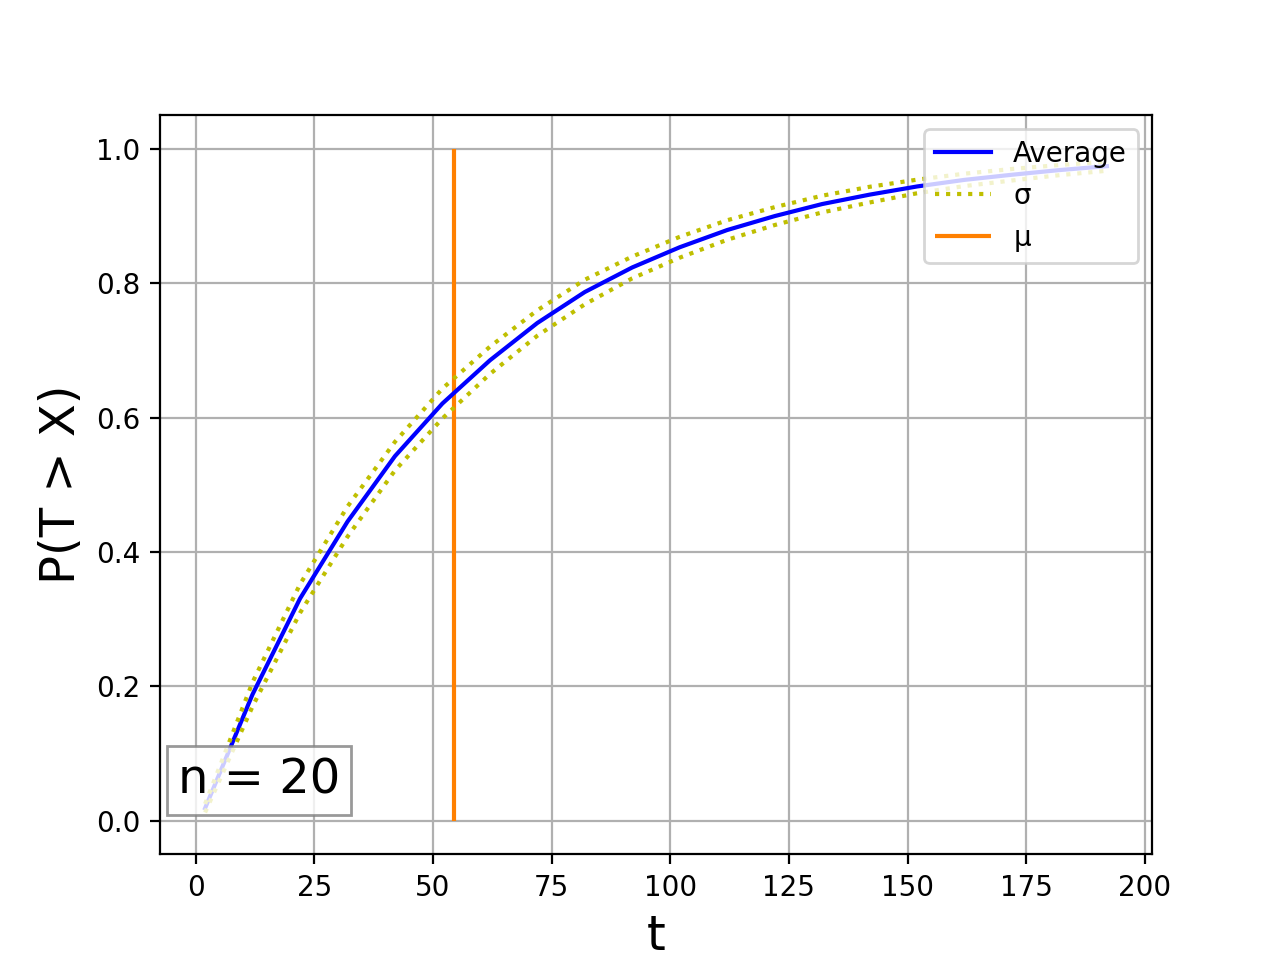
\includegraphics[width=1\linewidth]{plot_T_bigger_X_20.png} \\ n = 20}
        \end{minipage}
        \hfill
        \begin{minipage}[h]{0.49\linewidth}
            \center{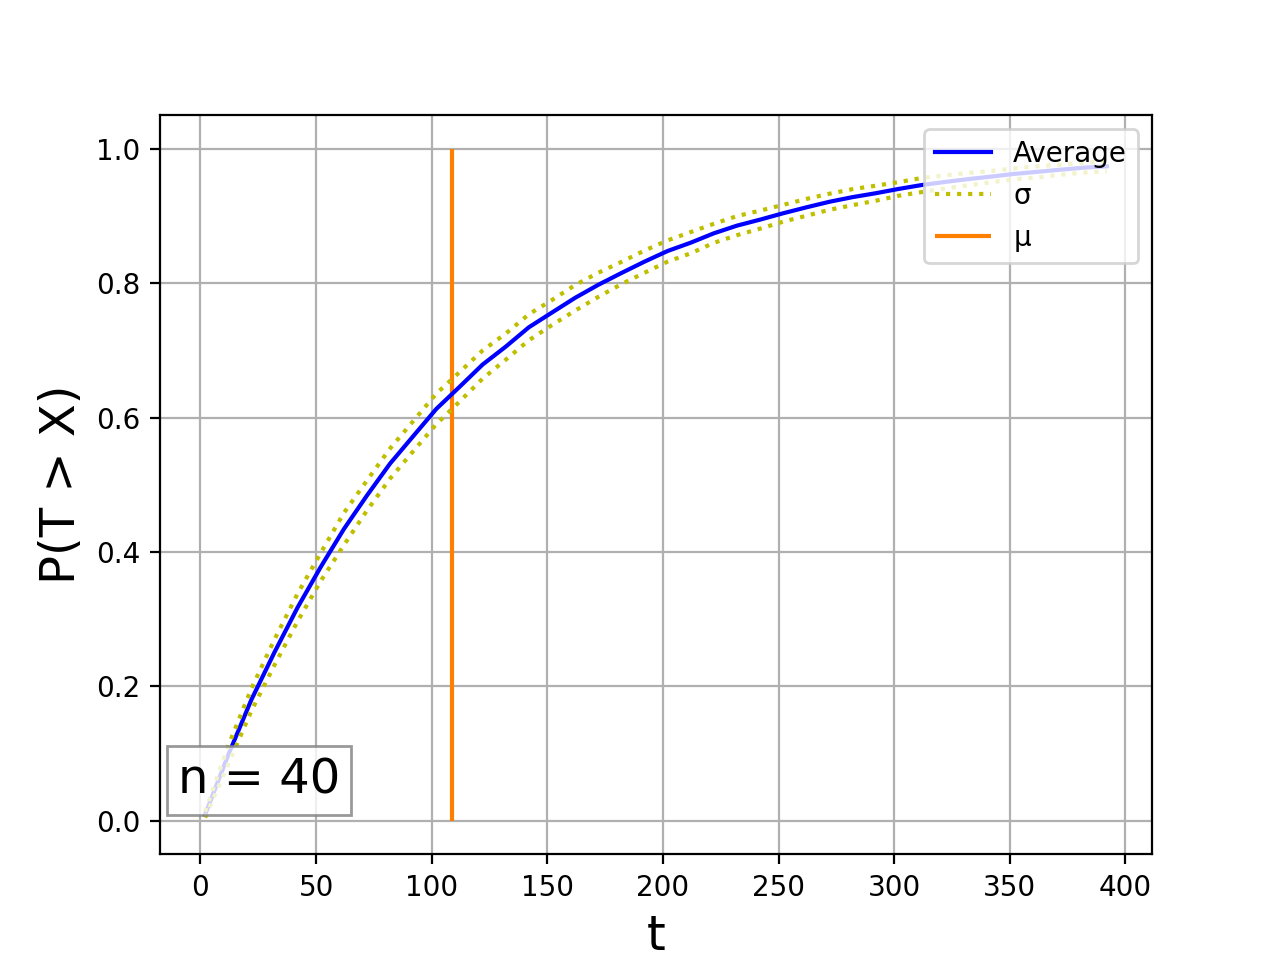
\includegraphics[width=1\linewidth]{plot_T_bigger_X_40.png} \\ n 200}
        \end{minipage}
        \caption{Как часто алгоритм найти успевает новый оптимум}
        \label{ris:image1}
    \end{figure}



    \begin{figure}[H]
        \centering
        \caption{Время работы алгоритма с n = 30}
        \label{pic:sublists-metafile}
        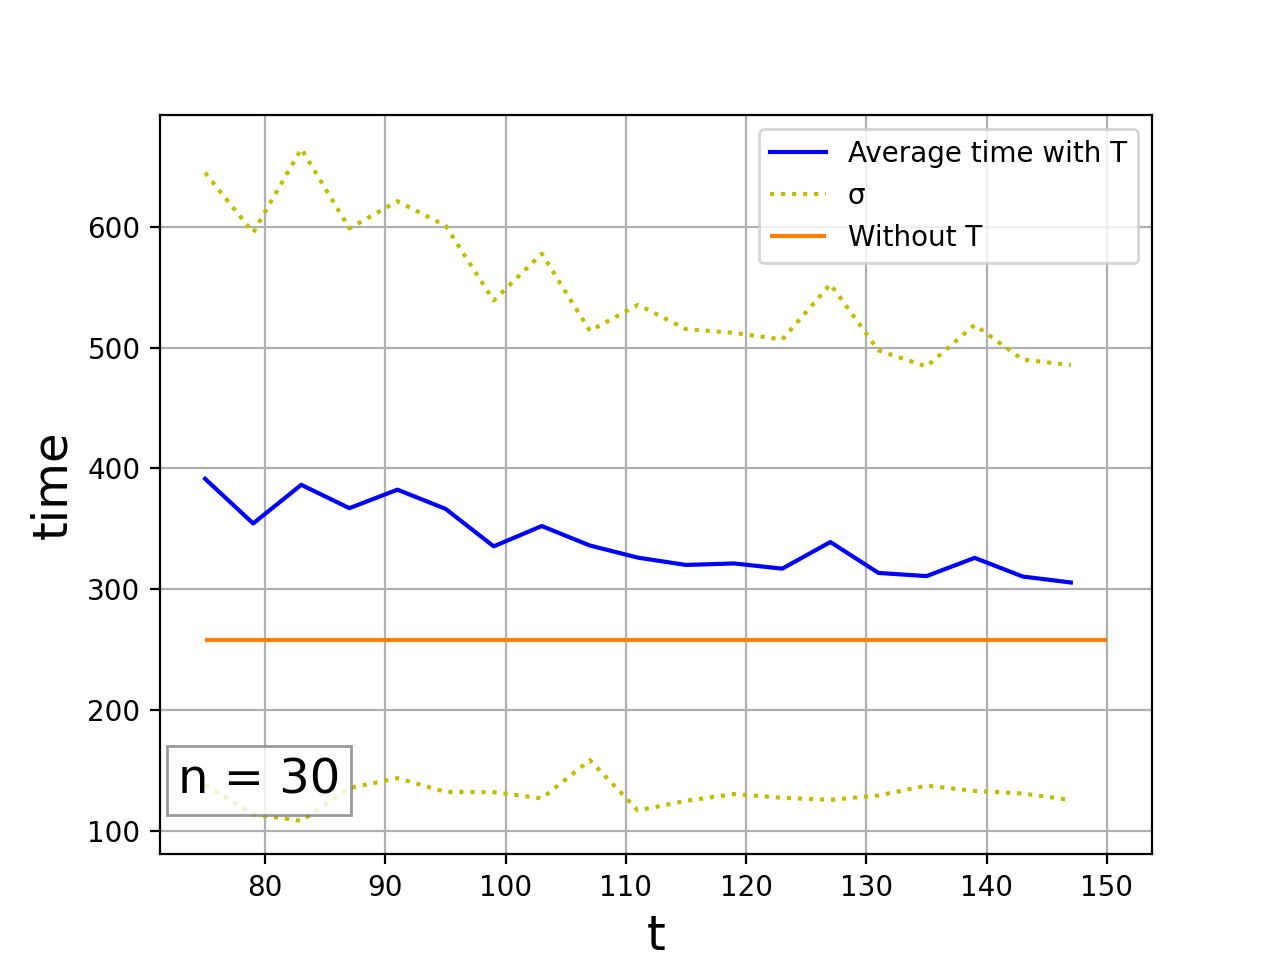
\includegraphics[scale=0.8]{plot_time_30_as_30.png}
    \end{figure}

    Для оценки скорости алгоритма рассматриваются разные значения $T$

    В качестве демонстрации основной гипотезы о независимости значения плато от $n$ поставлены несколько экспериментов с разными $n$, но с одной и той же $T = 10$. \\
    На графиках изображено усредненное поведение функции $d$ - количество разных бит у $x$ и $x^{opt}$ за 20 запусков. \\
    Как видно из экспериментов они все останавливаются примерно на одном уровне по отношению к $n$. \\

    \begin{figure}[h]
        \begin{minipage}[h]{0.49\linewidth}
            \center{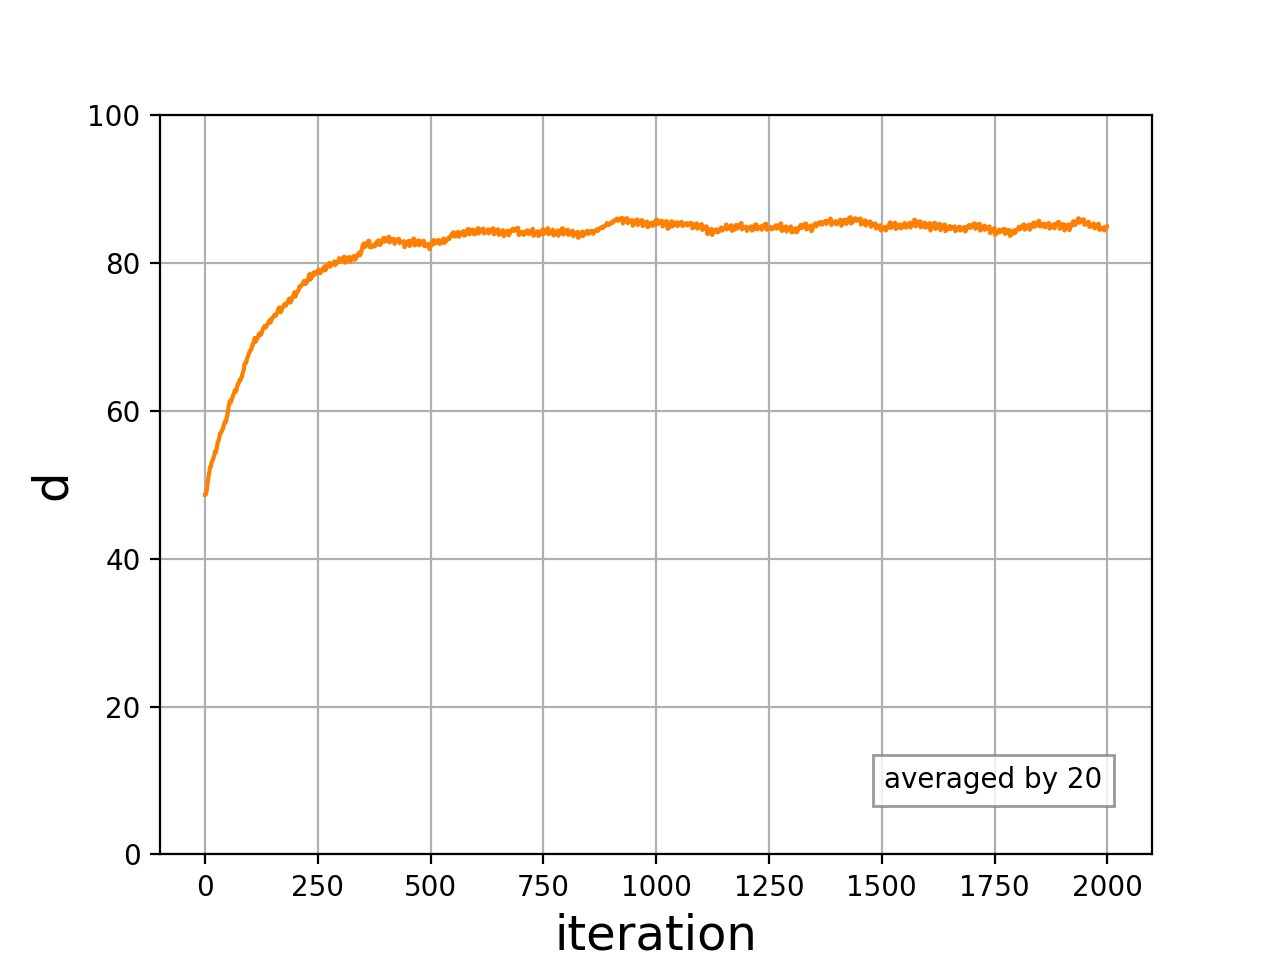
\includegraphics[width=1\linewidth]{plot_d_averaged_one_max_100_1_10_2000_20.png} \\ n = 100}
        \end{minipage}
        \hfill
        \begin{minipage}[h]{0.49\linewidth}
            \center{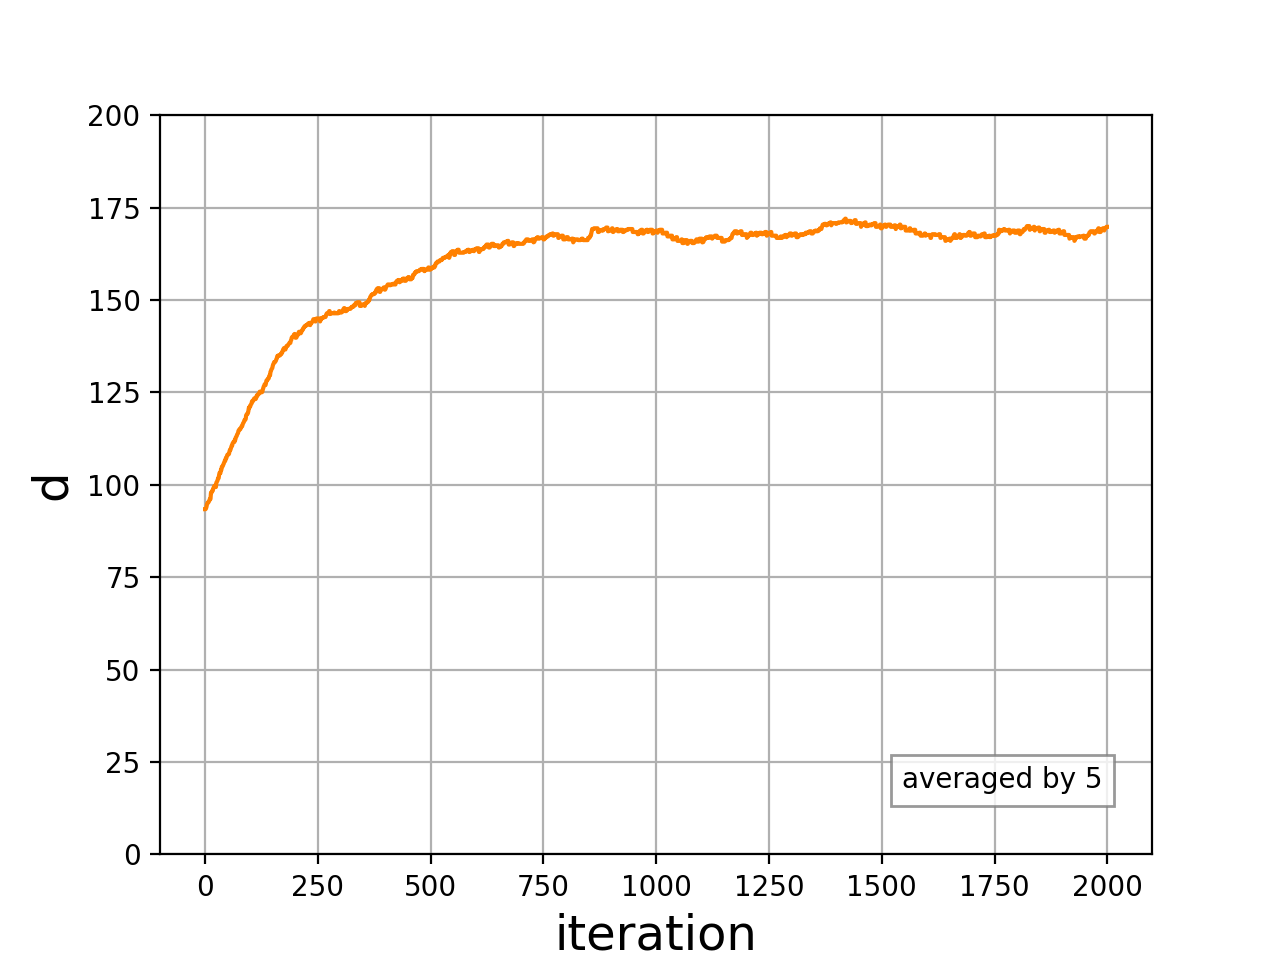
\includegraphics[width=1\linewidth]{plot_d_averaged_one_max_200_1_10_2000.png} \\ n 200}
        \end{minipage}
        \caption{Усредненное поведение алгоритма по 20 итерациям при T = 10}
        \label{ris:image1}
    \end{figure}

    \begin{figure}[h]
        \begin{minipage}[h]{0.49\linewidth}
            \center{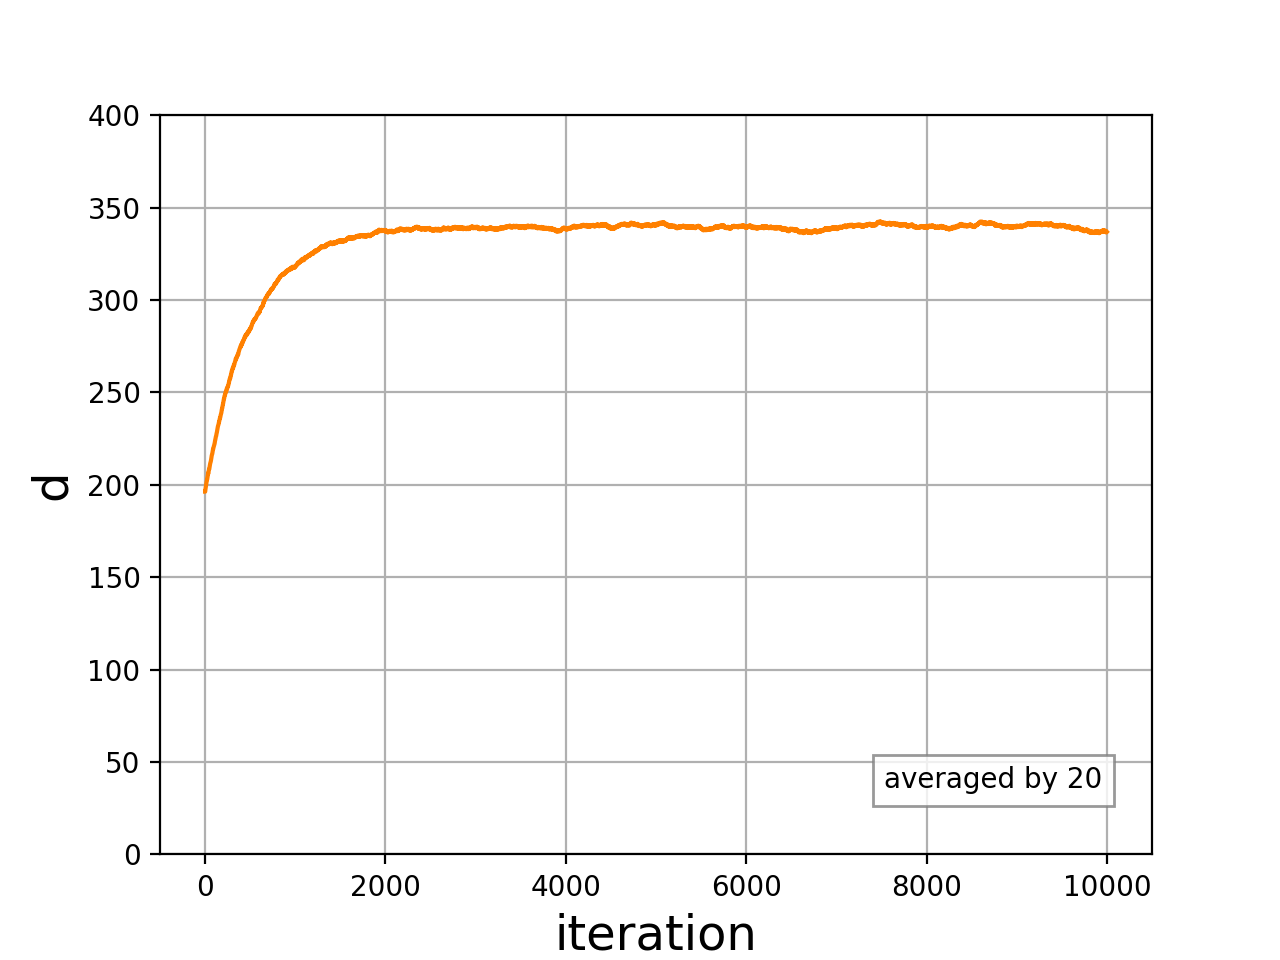
\includegraphics[width=1\linewidth]{plot_d_averaged_one_max_400_1_10_10000_20.png} \\ n = 100}
        \end{minipage}
        \hfill
        \begin{minipage}[h]{0.49\linewidth}
            \center{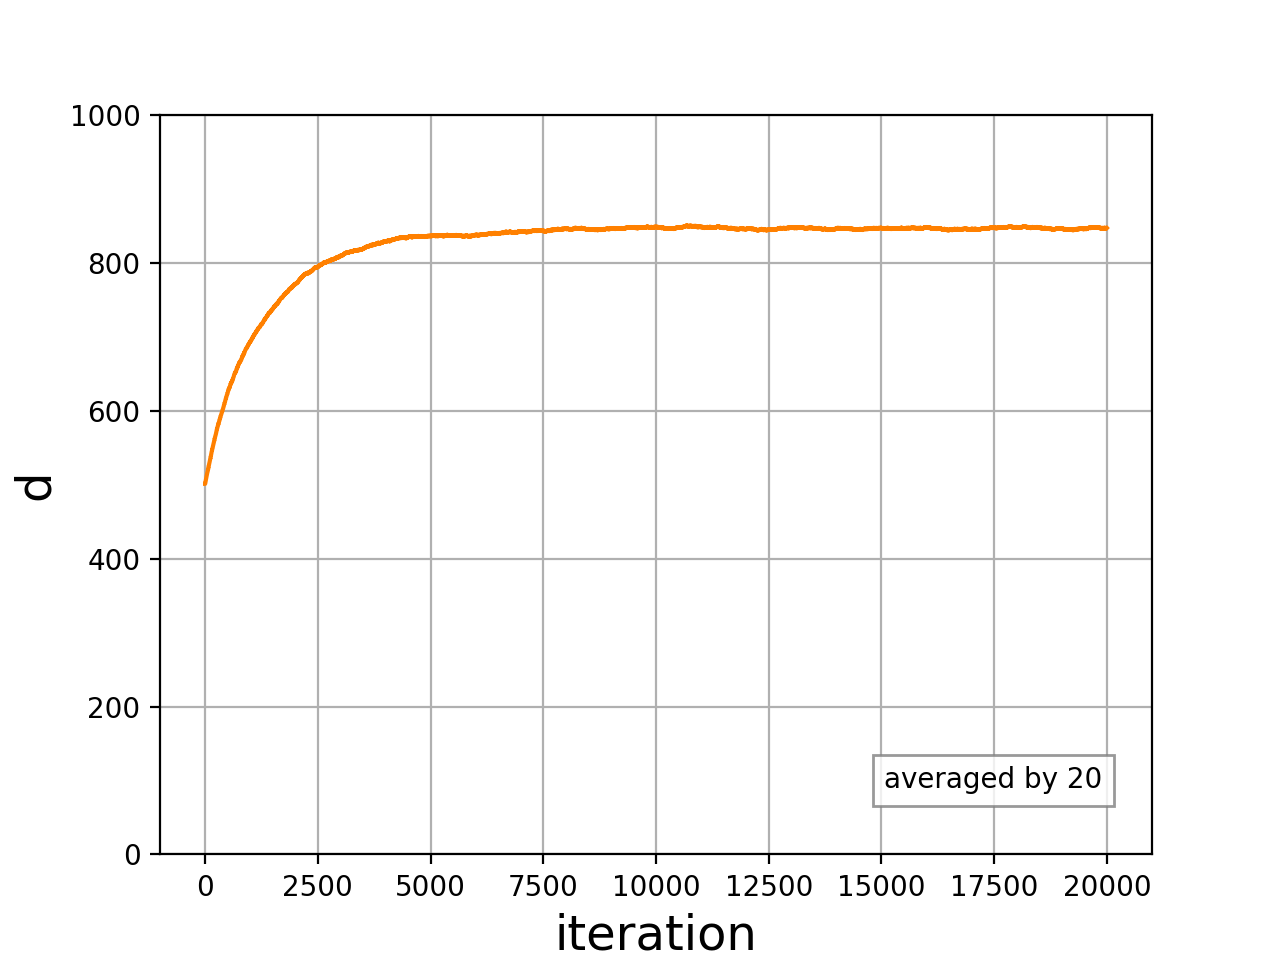
\includegraphics[width=1\linewidth]{plot_d_averaged_one_max_1000_1_10_20000_20.png} \\ n = 200}
        \end{minipage}
        \caption{Усредненное поведение алгоритма по 20 итерациям при T = 10}
        \label{ris:image1}
    \end{figure}
    \newpage
    В рамках анализа поведения было установлено, что если бы мы решали обратную задачу, то есть для данного $c$, пытались бы найти $T$, то оно лежало бы в промежутке $(g_{lower}, g_{upper})$  где $g_{lower}= \frac{(1 - c)}{\exp(-r + r\cdot c) \cdot c \cdot r}$; $g_{upper}(c) = \frac{(1 - c)}{\exp(-r + r\cdot c) \cdot c \cdot r \cdot (1 + \exp(-r\cdot c) \cdot c \cdot r^2)}$ так что для нахождения. $T$ взять обратную функцию от данной
    Для анализа функций $g_{upper}$ и $g_{lower}$ приведены следующие графики:

    \begin{figure}[h]
        \begin{minipage}[h]{0.49\linewidth}
            \center{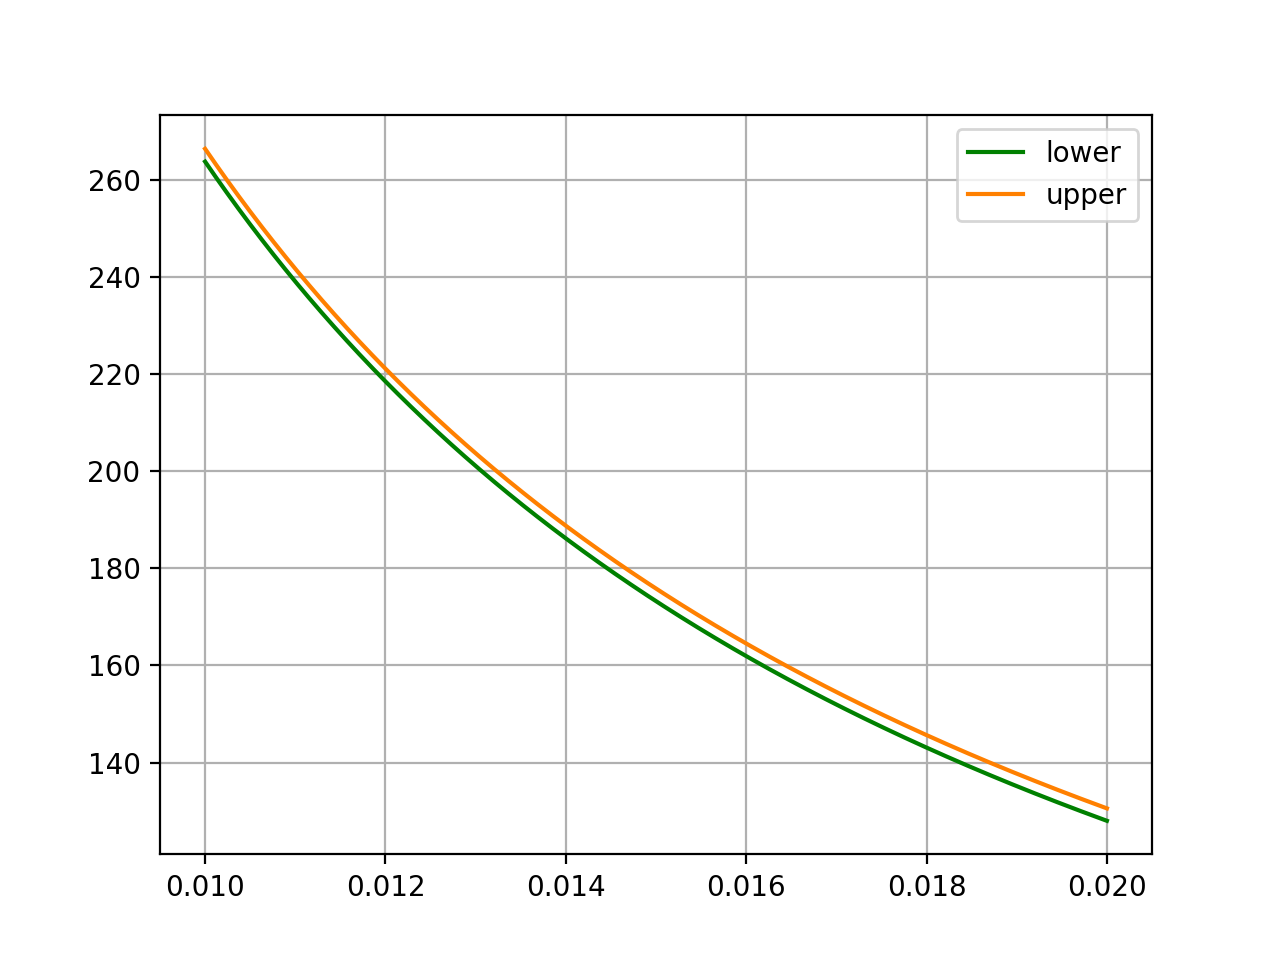
\includegraphics[width=1\linewidth]{kf_01_02.png} \\ с от 1 до 2}
        \end{minipage}
        \hfill
        \begin{minipage}[h]{0.49\linewidth}
            \center{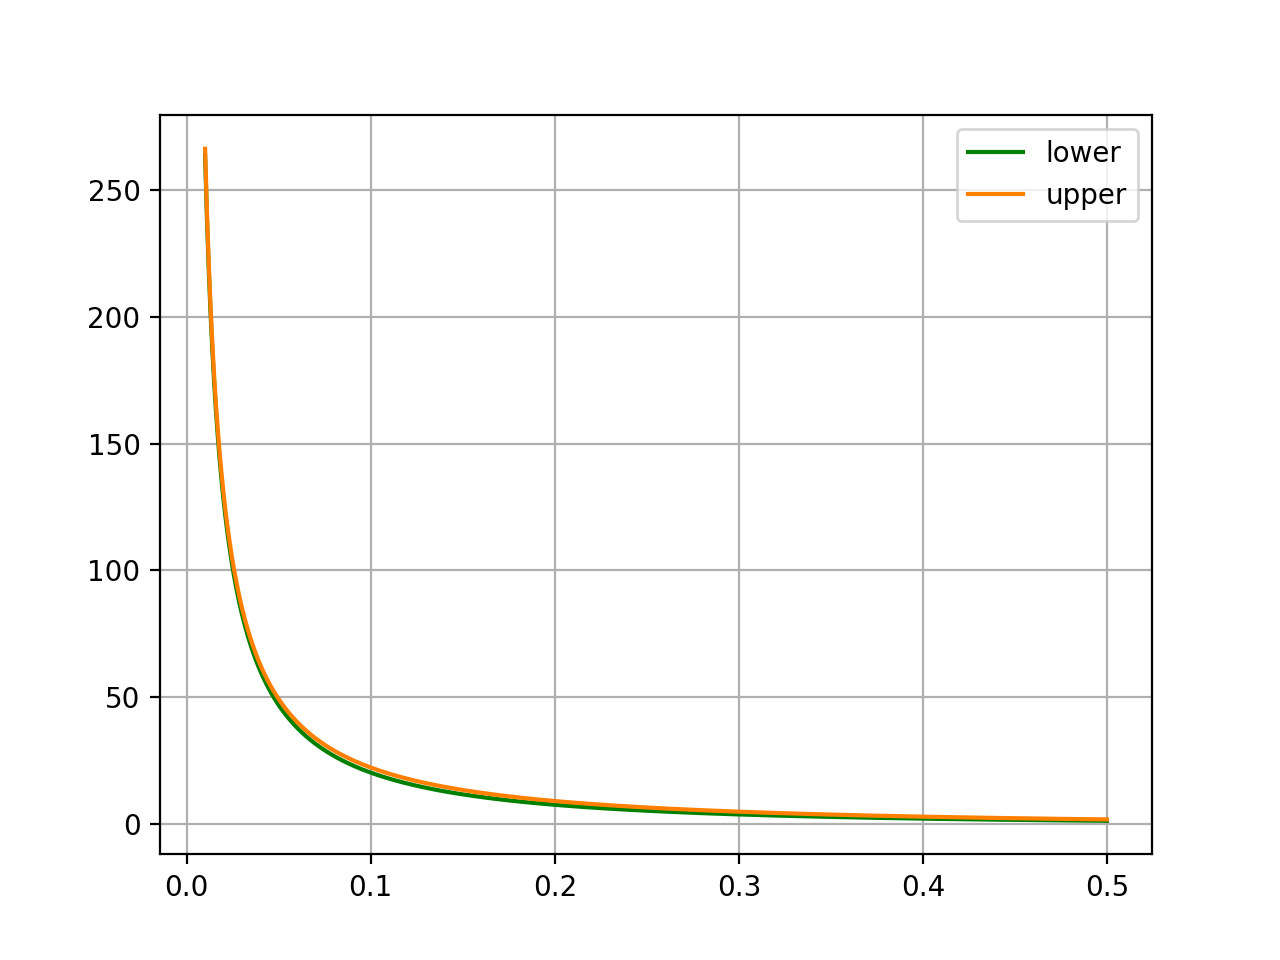
\includegraphics[width=1\linewidth]{kf_01_5.png} \\ с от 1 до 5}
        \end{minipage}
        \caption{Зависимость T от с}
        \label{ris:image1}
    \end{figure}

    \begin{figure}[h]
        \begin{minipage}[h]{0.49\linewidth}
            \center{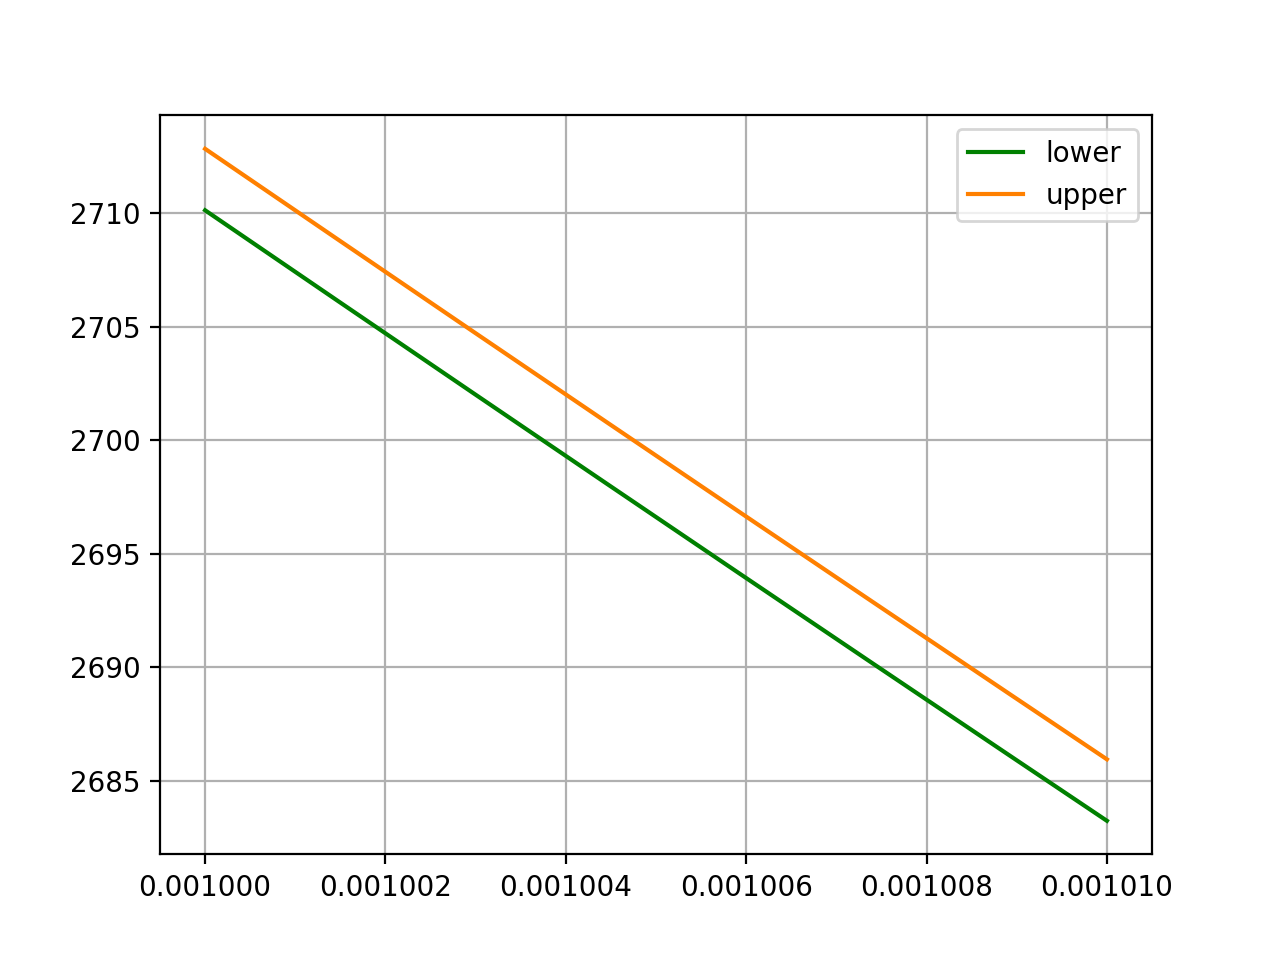
\includegraphics[width=1\linewidth]{kf_0001_00101.png} \\ с от 0.001 до 0.00101}
        \end{minipage}
        \hfill
        \begin{minipage}[h]{0.49\linewidth}
            \center{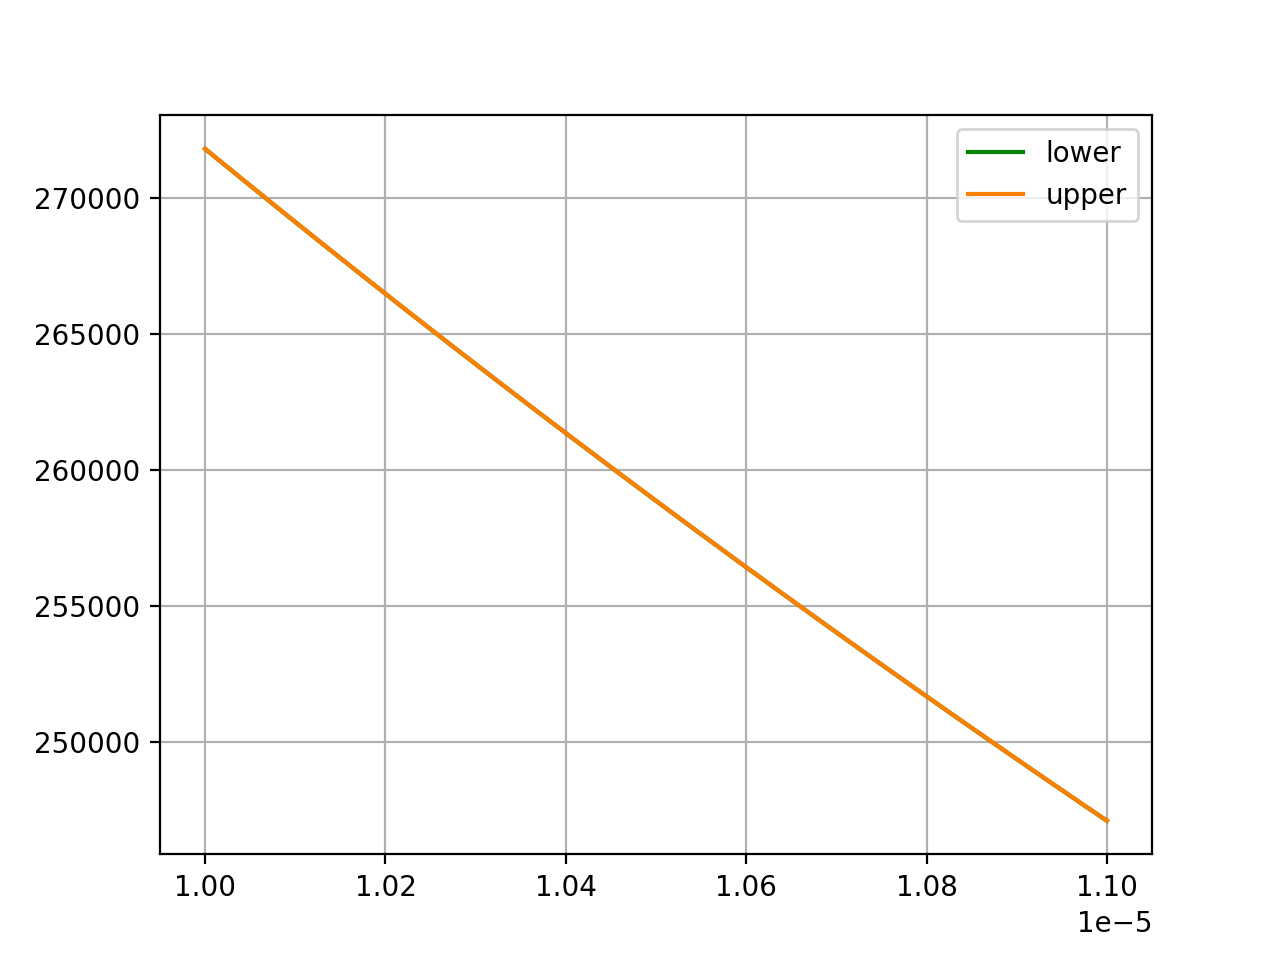
\includegraphics[width=1\linewidth]{kf_00001_000011.png} \\ с от 0.0001 до 0.00011}
        \end{minipage}
        \caption{Зависимость T от с}
        \label{ris:image1}
    \end{figure}

    \newpage
    Рассмотрим как предсказанная функция ведёт себя на практике
    \begin{figure}[h]
        \begin{minipage}[h]{0.49\linewidth}
            \center{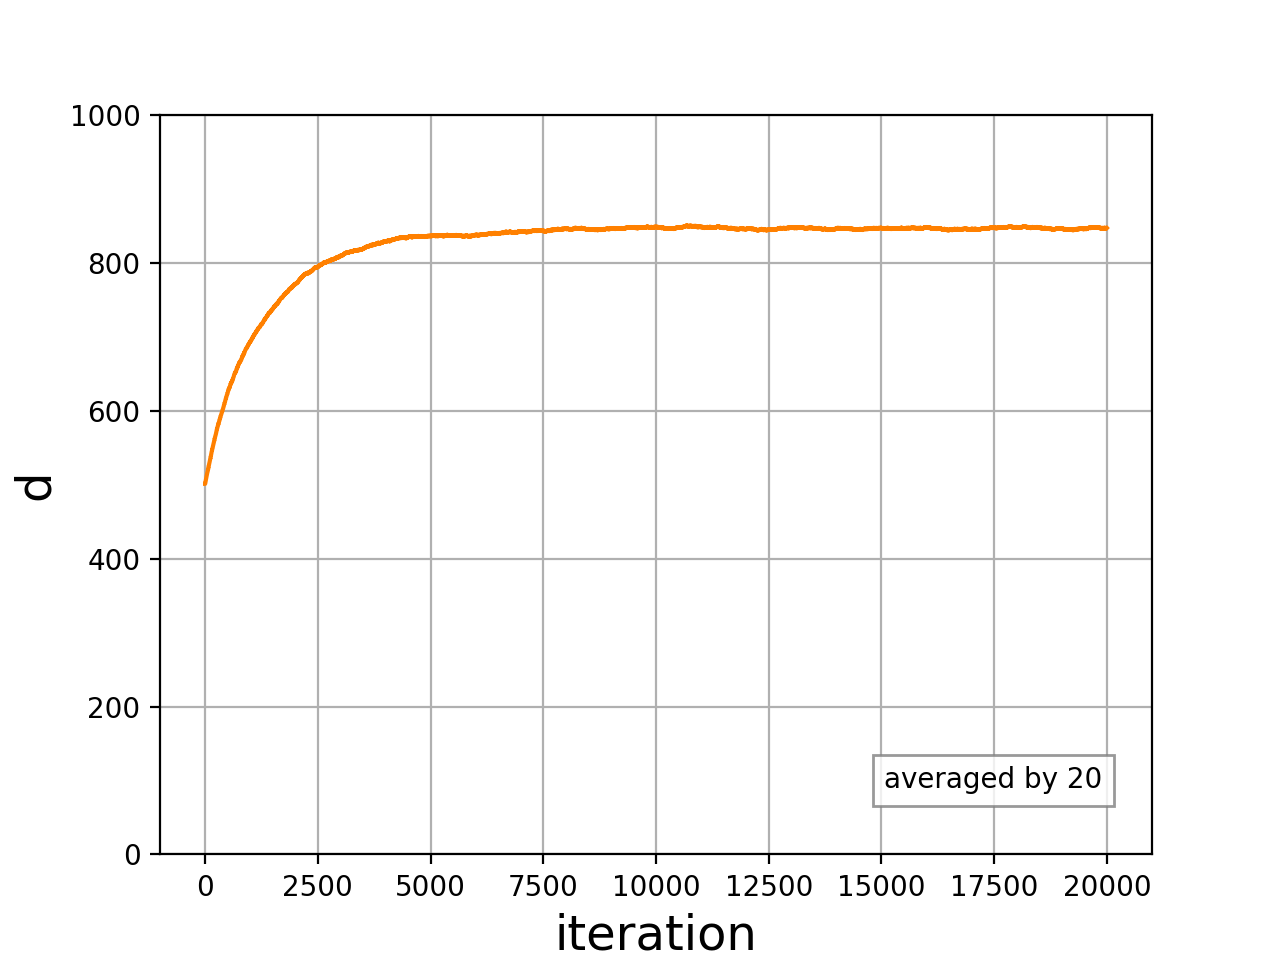
\includegraphics[width=1\linewidth]{plot_d_averaged_one_max_1000_1_10_20000_20.png} \\ Усреднённое значение по 20 итерациям}
        \end{minipage}
        \hfill
        \begin{minipage}[h]{0.49\linewidth}
            \center{\includegraphics[width=1\linewidth]{kf_005_030.png} \\ с от 0.05 до 0.30}
        \end{minipage}
        \caption{Анализ качества предсказанной функции}
        \label{ris:image1}
    \end{figure}

    Если взять значение из графика справа, то для $T = 10$ значение $c$ должно быть равно примерно 0.17, то есть остановиться на $1000 \cdot (1 - 0.17) = 830$, что и показывается на практике.

    \startconclusionpage
    В результате были сформуилорованы и доказаны несколько теорем, которые помогут в дальнейшим анализировать эволюционные алгоритмы с динамическими изменениями.
    Даны оценки кака точка стабилизация будует находиться для данного T. То есть в каком месте алгоритм будет находиться в независимости от n.
    Выведены пару drift-теорем, которые могут помочь дальнейшим исследованиям динамических оптимизаций, в частности теоремы применены к данной задаче в следствие чего была установлены такие значение T, при которых алгоритм будет находить оптимумы за то же асимптотическое время.
    Оценки были подтверждены экспериментальными данными.
    \printmainbibliography


\end{document}
